\documentclass[border=10pt]{standalone}

\usepackage{pgfplots}
\usepackage{tikz}
\usetikzlibrary{positioning, shapes.geometric, arrows}
%\pgfplotsset{compat=1.8}
%\usepgfplotslibrary{fillbetween} %for fill under curve

%\def\myellipse{(0,0) ellipse (2cm and 1cm)}
\renewcommand{\vec}[1]{\textbf{#1}}

\tikzstyle{gkreis} = [circle, draw=black, fill=green!30]

\tikzstyle{rkreis} = [circle, draw=black, fill=red!30]

\tikzstyle{bkreis} = [circle, draw=black, fill=blue!30]

\tikzstyle{arrow} = [->,>=stealth]






\begin{document}

    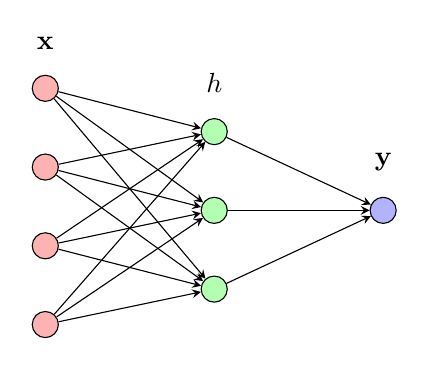
\begin{tikzpicture}[node distance=1cm]
    	
    	\node [rkreis] (11) {};	
 		\node[above=of 11, yshift=-0.8cm] (01) {$\vec{x}$};
 		\node[right=of 01, xshift=-1cm, yshift=-0.22cm] (001) {};	
 		\node[right=of 01, xshift=-0.9cm, yshift=-0.25cm] (002) {};	
 		\node[right=of 01, xshift=-0.5cm, yshift=-0.5cm] (003) {};
    	\node [rkreis, below of=11] (12) {};
    	\node [rkreis, below of=12] (13) {};
    	\node [rkreis, below of=13] (14) {};
    	%\node [rkreis, below of=14] (15) {};
    	
	
    	\node [gkreis, right=of 11, yshift=-0.55cm, xshift=0.8cm ] (21) {};
    	\node[above=of 21, yshift=-0.8cm] (01) {$h$};
    	\node [gkreis, right=of 12, yshift=-0.55cm, xshift=0.8cm ] (22) {};
    	\node [gkreis, right=of 13, yshift=-0.55cm, xshift=0.8cm ] (23) {};
    
    	\node [bkreis, right=of 22, xshift=0.8cm ] (31) {};
    	\node[above=of 31, yshift=-0.8cm] (01) {$\vec{y}$};
    	
    	%\draw[arrow] (001) -- (23);
    	%\draw[arrow] (002) -- (22);
    	%\draw[arrow] (003) -- (21);
    	
    	\draw[arrow] (11) -- (21);
    	\draw[arrow] (11) -- (22);
    	\draw[arrow] (11) -- (23);
    	
    	\draw[arrow] (12) -- (21);
    	\draw[arrow] (12) -- (22);
    	\draw[arrow] (12) -- (23);
    	
    	\draw[arrow] (13) -- (21);
    	\draw[arrow] (13) -- (22);
    	\draw[arrow] (13) -- (23);
    	
    	\draw[arrow] (14) -- (21);
    	\draw[arrow] (14) -- (22);
    	\draw[arrow] (14) -- (23);
    
    	%\draw[arrow] (15) -- (21);
    	%\draw[arrow] (15) -- (22);
    	%\draw[arrow] (15) -- (23);
    	
    	\draw[arrow] (21) -- (31);
    	\draw[arrow] (22) -- (31);
    	\draw[arrow] (23) -- (31);
    	
    \end{tikzpicture}

\end{document}
